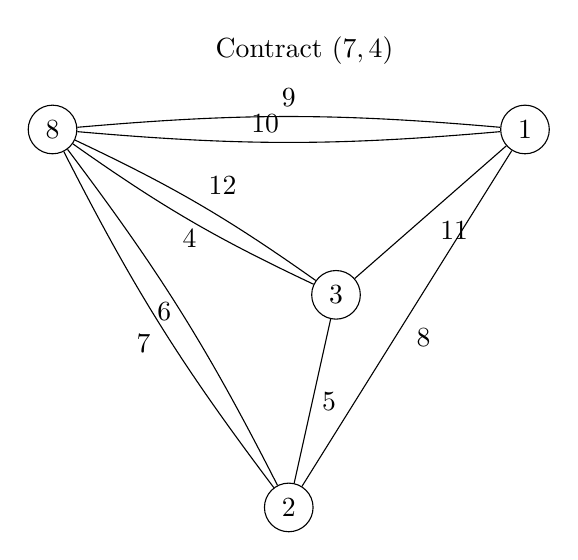
\begin{tikzpicture}
	\node (G) at (2, 1) {Contract $(7,4)$};
	% Define the nodes with specific positions
	\begin{scope}[xshift=0cm, yshift=0cm, scale=0.6]
		\node[circle, draw] (1) at (8, -0) {1};
		\node[circle, draw] (2) at (3, -8) {2};
		\node[circle, draw] (3) at (4, -3.5) {3};
		\node[circle, draw] (8) at (-2, -0) {8};
	
		% Draw the edges between nodes with labels
		\draw[draw] (3) to[bend left=5] node[below] {4} (8);
		\draw[draw] (3) -- node[right] {5} (2);
		\draw[draw] (8) to[bend left=5] node[left] {6} (2);
		\draw[draw] (2) to[bend left=5] node[below left] {7} (8);
		\draw[draw] (1) -- node[below right] {8} (2);
		\draw[draw] (1) to[bend right=5] node[above] {9} (8);
		\draw[draw] (1) to[bend left=5] node[above left] {10} (8);
		\draw[draw] (1) -- node[below right] {11} (3);
		\draw[draw] (8) to[bend left=5] node[above right] {12} (3);
	\end{scope}
\end{tikzpicture}